\documentclass[12pt,a4paper]{scrartcl}
\usepackage[utf8]{inputenc}
\usepackage[german]{babel}
\usepackage{wrapfig}
\usepackage{graphicx}
\usepackage{amsmath}
\usepackage[justification=centering]{caption}

\begin{document}

\section{Simulation und Darstellung der Ultraschallprüfung}
Die Simulation der Scanverfahren und die finale Berechnung und Auswertung der Reflexionen wird in der Klasse \textsc{Scan} umgesetzt. %%todo einheitlich Klassen anders

\subsection{Raytracer und und die trace-Funktion}
Die im vorangegangenen Kapitel hergeleiteten Formeln sind in der Klasse \texttt{Raytracer} implementiert. Daher existiert für jede geometrische Form eine Methode zum Berechnen des Schnittpunktes mit dem Strahl und eine zur Berechnung des reflektierten Vektors und somit des neuen Strahls. Weiterhin gibt es spezielle Prozeduren um das Problem der Reflexion in einer Ecke zu behandeln.\\
Das Kernstück der Klasse ist jedoch die \texttt{trace}-Funktion, welche dazu dient, den gesamten Verlauf eines Strahls im Probekörper zu ermitteln. Dazu wird mithilfe der Schnittpunkt-Funktionen der Schnittpunkt mit jedem Objekt in dem Körper ermittelt, sofern existent. Anschließend wird die Reflexionsmethode für dasjenige Objekt aufgerufen, welches tatsächlich vom Strahl getroffen wird, also dessen Schnittpunkt mit dem Strahl am nächsten an dem Ausgangspunkt des Strahls liegt. Sind mehrere Objekte gleich weit entfernt, wird die Funktion zur Reflexion an Ecken aufgerufen, sodass in jedem Fall ein eindeutiger neuer Strahl entsteht.\\
Bei jeder einzelnen Reflexion wird der vorherige Strahl in einer Liste gespeichert, sodass am Ende sämtliche Strahlen mit Anfangspunkt und Richtungsvektor geordnet in dieser Liste stehen. Mithilfe dessen ist der Verlauf des Strahls durch den Prüfkörper eindeutig nachvollziehbar, indem die Reflexionspunkte in der gegebenen Reihenfolge betrachtet werden.

\subsection{Scanverfahren}
%%todo Anknüpfen an Text davor, Bezug auf Klassen selbst oder algorithmische Erklärung der Verfahren?
Basierend auf den von Raytracer ermittelten Punkten, an welchen die Strahlen reflektiert werden, errechnet man, welche Zeit zwischen den einzelnen Reflexionen vergeht.
Weiterhin wird für jeden Auftreffpunkt geprüft, ob dieser im Messbereich des Senders liegt. 
Ist dies der Fall, so wird in Abhängigkeit der bereits verstrichenen Zeit die Intensität ermittelt. 
Insgesamt geht man hierbei von einer über die Zeit exponential fallenden Intensität aus.\\
Ähnlich verhält es sich auch bei der Simulation mit mehreren Strahlen. 
Hierfür werden die Strahlen gleichmäßig über den gegebenen Streuwinkel verteilt und für jeden Strahl die zuvor erklärte Prozedur durchgeführt. 
Final werden alle ermittelten Wertepaare aus Zeit und Auftreffintensität zusammengefasst.\\
Das Verfahren kann dabei von zwei verschiedenen Größen abhängig gemacht werden. 
Zum einen der maximalen Anzahl an Reflexionen, die für alle Strahlen gleichermaßen festgelegt wird. Hierbei liegt der Vorteil darin, dass die benötigte Speichermenge und Rechenzeit limitiert ist und vom Benutzer besser gesteuert werden kann. 
Nachteilig ist hingegen, dass einzelne Strahlen, die in einem engen Bereich zwischen zwei begrenzenden Flächen oft reflektiert werden damit insgesamt kürzere Strecken zurücklegen, als Strahlen die nur auf den Begrenzungsflächen des Prüfkörpers auftreffen. 
Dies führt zu eventuellen Verlusten von Messwerten, die in einer realen Anwendung wahrnehmbar gewesen wären, da die Strahlen mit kürzerem Weg noch eine höhere Intensität haben und eventuell nach weiteren Reflexionen den Sender noch erreichen könnte.\\
Um diesen Fall ebenfalls abzudecken ist eine zweite Version dieser Prozedur verfasst. 
Hierfür wird statt einer maximalen Anzahl an Reflexionen die maximale Weglänge eingelesen. 
Damit legt jeder Strahl im Material die gleiche, vom Benutzer ausgewählte Strecke zurück, womit das Problem von Messwertverlusten gelöst wird. 
Der Nachteil hierbei liegt allerdings darin, dass man für einen Strahl nie voraussehen kann, wann die Maximalweglänge überschritten wird. 
Daher kann es hierbei zu einer hohen Anzahl an Reflexionen kommen, welche proportional zu Speicherbedarf und Rechenzeit sind. 
Insgesamt muss hier für jeden Anwendungszweck separat entschieden werden, welchen Verfahren mit seinen Vor- und Nachteilen gewählt wird.\\


\newpage
\subsection{Auswertung der Scanergebnisse}
%%todo verweis Struktogramm Anhang
Ungeachtet des gewählten Verfahrens kommt es bei der Darstellung der Messwerte eines Scans der auf einem Strahlenbündel basiert immer zu dem Problem, dass Strahlen die einen ähnlichen Verlauf haben sehr kleine zeitliche Differenzen zwischen ihrem Auftreffen auf dem Sender haben. 
In der Nebenstehenden Abbildung \ref{fig:Wegunterschied} zu erkennen ist sind die zurückgelegten Strecken und damit die benötigte Zeit der einzelnen Strahlen, besonders wenn man noch kleinere Streuwinkel wählt, gering.
%%todo bild kleines senkrechtes Bündel  zur Veranschaulichung
\begin{wrapfigure}{H}{2.8cm}
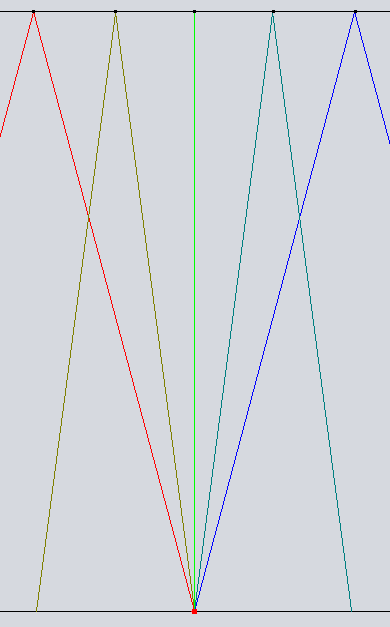
\includegraphics[scale=0.25]{pictures/Strahlenbuendel.png}
\label{fig:Wegunterschied}
\caption{Strahlenverlauf}
%%todo caption
\end{wrapfigure}
Die im Diagramm dargestellten Werte überlappen sich, doch dies entspricht nicht der Realität. 
Durch die Annahme, dass jeder Strahl einen gewissen Teil der kinetischen Energie, die in Form der Schallwelle in den Körper abgegeben wird, repräsentiert sollten fast gleichzeitige Treffer nicht als solche wahrgenommen werden, sondern als ein Treffer mit höherer Intensität. %%todo ohne erklärung Welle?
Die Notwendigkeit einer weiteren Zusammenfassung der Messwerte ist dadurch gegeben. 
Dies erfolgt in der Methode \textsl{processScan}. %%todo einheitliche Schriftart für funktionen, Satz notwendig?
\begin{wrapfigure}{L}{11.5cm}
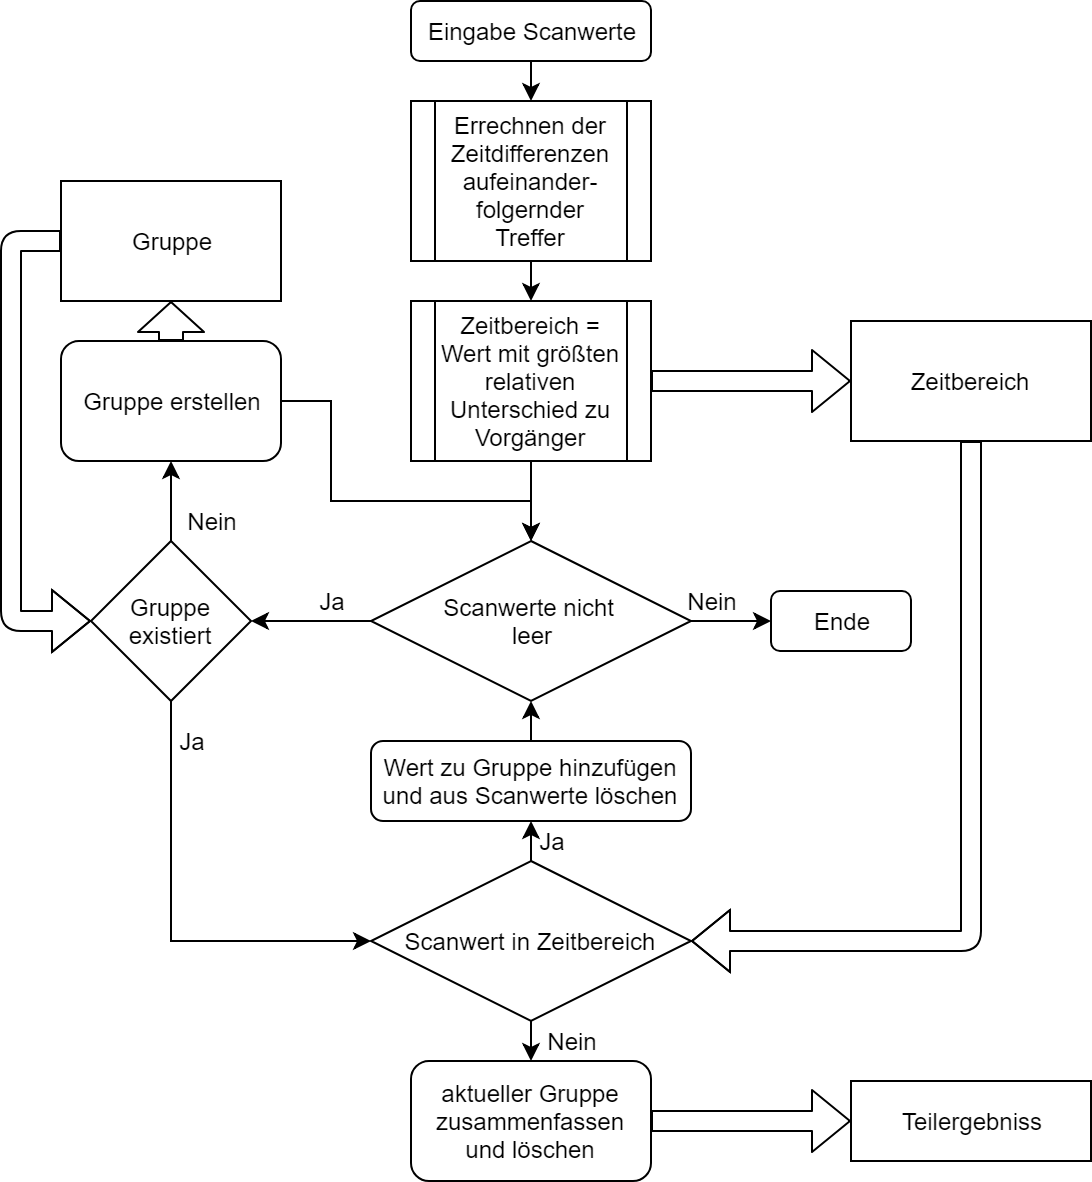
\includegraphics[scale=0.3]{pictures/Flowchart_processScan.png}
%%todo caption
\end{wrapfigure} \par
Zuerst werden dabei alle Wertepaare aus Zeit und Intensität errechnet und in zeitlicher Abfolge sortiert. 
Zwischen zwei Wertepaaren liegt eine Zeitdifferenz, die für alle Paare errechnet wird und in eine Liste einsortiert wird.
Nun wird aus dieser Liste an Differenzen die Stelle gesucht, an der der Quotient aus zwei aufeinanderfolgenden Zeitdifferenzen am größten ist und der größere Wert der Zeitdifferenzen als sogenannter Zeitbereich definiert. 
Dieser sagt aus, in welchen Abstand von einem gegebene Treffer weitere Treffer nicht separat in das Diagramm für A-Scans eingetragen, sondern als ein Treffer zusammengefasst werden.\\
Auf Basis des Zeitbereichs werden nun alle Scanwerte durchgegangen und in Gruppen eingeteilt. 
Ausgehend von einem Startwert werden alle folgenden Werte überprüft und solang der selben Gruppe zugeordnet, bis sie nicht mehr innerhalb des Zeitbereichs liegen. 
Die Gruppe wir dann ausgewertet, indem eine durchschnittliche Intensität der Treffer sowie eine Durchschnittszeit errechnet wird. 
Dieses Teilergebnis ist eines der neuen Wertepaare, welche dann im Diagramm für A-Scans dargestellt werden. 
Die Gruppe wird daraufhin geleert, ein neuer Wert hinzugefügt und das Verfahren wiederholt bis alle Scanergebnisse einer Gruppe zugeordnet wurden.


\end{document}